\lab{Python}{Data Structures I}{Data Structures I}
\label{lab:Python_DataStructures}
\objective{Learn about data structures}

We can store data in computer in a variety of ways.
The most basic way we have to store data is via primitive datatypes.
These datatypes are booleans, strings, floats, and integers.
Most information that we care to store is in one of these forms.
However, for storing large amounts information, these primitive types can quickly become unwieldy.
We can create more natural ways to store data.  We use these primitive datatypes as building blocks along with arrays (or lists in Python).  
The more complex data structures are called \emph{abstract data types}.
Python has a couple of the more common abstract data types such as dictionaries, sets, and lists.
All of the abstract data types slow down in performance as the size of the data structure increases.

Most abstract data types use an object called a \emph{node} to store data.
A node essentially acts as a box in which we store an arbitrary piece of data.
A good analogy is to think of a postal delivery system as an abstract data structure.
We start by inserting an item into the system.  This item can be anything.
The first thing that the postal system will do is put the item in a box.
The postal system now only has to efficiently handle boxes.
It doesn't have to worry about working with each item that goes through system.
They postal system can attach delivery specific data to any box that allow it to be processed more effectively.
A postal system has abstracted itself from the items it delivers.
If we didn't use nodes, or data boxes, we would have to build a new tree for each datatype we wanted to store.
Nodes allow us to abstract data structure from the kind of data we wish to store.
A node in a binary tree will be different from a node used in a priority queue.
Nodes allow us to generalize the functionality of a data structure.

\section*{Linked Lists}
Linked Lists are one of the most basic and common data structures.
Linked lists use nodes to store data and are linked together.
Nodes can be inserted or removed from either end in a constant amount of time, independent of the size of the list.
To insert or delete nodes in the middle of the list, the correct node must first be located.  
Finding this node requires traversing the list which will take longer as the list size grows.  
Linked lists do not allow random access like arrays.  
Linked lists always have a reference that points the head, or first node, of the list.  
They may also have a tail reference that will point to the end, or last node, of the list.

There are several ways we can link the nodes together.  The three most common ways are singly-linked, doubly-linked, and circularly-linked.  
Singly-linked nodes store only a single reference that points to the next node in the list.  
Doubly-linked nodes have two references that point point the previous and next nodes in the list.  
This allows for a doubly-linked list to be traversed in both directions, whereas a singly-linked list can only be traversed in one direction. 
A circularly linked list is a singly or doubly-linked list where the tail node points to the head node as the next node.  
Circularly-linked lists are commonly used as data buffers.

\begin{problem}
Implement a singly-linked list with methods for inserting, removing, and finding nodes.  You should also implement a method that clears the list.
\end{problem}

\section*{Hash Tables}
A hash table is a very simple data structure that trades space for speed.
Most operations of a hash table execute in constant time, independent of the size of the data structure.  
They have very fast lookup times.  They form the underlying data structure of Python's dictionaries.

The heart of a hash table is a good hash function.  
A hash function maps an input to a positive integer. 
This positive integer is then used as an index to access the hash table. 
Since the hash function must be executed to perform any operation on the hash table, it is important that the hash function executes quickly.
An ideal hash function will map a unique inputs to unique outputs that are uniformly distributed over the hash space. 
However, it is very difficult to make a perfect hash function.  Most hash functions will experience \emph{hash collisions}. 
This is where two unique inputs yield the same hash output.
There are ways of handling hash collisions.  The two methods that we will discuss are open addressing and chaining.

\subsection*{Open Addressing}
Open addressing means that the output of the hash function doesn't necessary identify the location of some data.
A popular form of open addressing is probing. 
We will discuss linear probing and quadratic probing.

In the event of a hash collision, linear probing seeks to resolve the collision by looking for the next available location in the hash table.
A linear probing hash function where $n$ is the size of the hash table, $h(x)$ is the hash function, and $i$ is a constant is of the form
\begin{equation*}
h(x, i) = h(x) + i \pmod{n}
\end{equation*}
We can do this by sequentially visiting each subsequent location and when we find an empty one, stuff our data in that location.  
However, when we want to retrieve that information, when we hash it, we will be directed to the wrong location. 
We then have to begin iterating through the table looking for our data.
If our hash table is densely populated or our hash function has lots of collisions, 
then we lose the efficiency of a hash table because we are forced to resort to a linear search.
With linear probing, elements in the table will cluster together.

Quadratic probing seeks to mitigate the issues of linear probing by spreading out hash collisions more evenly.   
A quadratic probing hash function where $c_1$ and $c_2$ are constants is of the form
\begin{equation*}
h(x, i) = h(x) + c_1i + c_2i^2 \pmod{n}
\end{equation*}

\subsection*{Chaining}
Chaining is a form of closed addressing.  The output of the hash function points the location of the data. 
With chaining, each location of the hash table references a list.
When one or more pieces of information hash to the same location, it is added to that location's list.  
With a good hash function, the average size of hash location's list is relatively short,
so searching the list doesn't affect the overall performance of the hash table.

\subsection*{Hash Table Details}
As a hash table fills up, its performance degrades.
When using a hash table, a \emph{load factor} is often tracked.
This load factor reveals how full the table is and by calculating the ratio of the number of empty locations to total number of locations in the hash table.
When the load factor exceeds a certain threshold, we must allocate more space for the table.
To allocate more space, we must re-hash everything in the table (since most hash functions are computed modulo the size of the table).
This can sometimes be a very expensive operation.
It's important to avoid resizing the table when possible.

\begin{problem}
Implement a hash table that uses chaining for resolving hash collisions.
When, the load factor exceeds $.75$, resize the hash table so that the load factor will be below $.33$.
\end{problem}

\section*{Trees}
Trees are a rooted group of linked nodes.  There are many types of trees, but we will only cover one of the most basic ones, the binary search tree.
The binary search tree will show us the basics elements of the tree data structure.
A binary tree is a tree that has a maximum of two children per node.
A binary search tree has the added properties that all there are no duplicate elements
and that the structure of the tree is ordered. 
A very common ordering is the left half of the tree contains elements less than the root, and the right contain elements greater than the root.

Searching a binary search tree is very fast.
The structure of the binary search tree mimics the execution of a binary search.
Due to the fact that locating a node in a binary search tree is very fast, inserting and removing nodes is also very fast.  
Binary search trees are often used to represent the elements of a set.

The node in a binary search tree holds a (key, value) pair and references to left and right subtrees. 
This is a recursive data structure because each of the left and right subtrees are themselves binary search trees.
\begin{lstlisting}
class Node(object):
    def __init__(self, data):
        self.data = data
        self.left = None
        self.right = None
\end{lstlisting}
Many of the algorithms for working with binary search trees are also recursive.
A recursive function is a function that calls itself until it reaches a base case.
In the search function below, the two base cases are either we have the correct
node, or we don't have a node at all. 
In both these cases, we just return what we have.
We don't have to use recursive algorithms if we don't want to.  In fact, for large trees, a recursive algorithm will consume a lot of resources.
\begin{lstlisting}
def search(data, node):
    if node is None or node.data == data:
        return node
    elif data < node.data:
        search(data, node.left)
    else:
        search(data, node.right)
\end{lstlisting}

Inserting a node into a binary search tree is simple procedure.
We recursively insert to the right if the element is greater than the current node
or insert on the left is the element is less than the current node.
We never insert a non-leaf node in a BST.

Removing nodes is only slightly more complicated.
We have three cases to consider.
\begin{itemize}
\item No child nodes.  This is the simplest case.  We simply remove the node.
\item One child node.  In this case, we have to worry about children.
The solution is simple enough. 
We promote the child to take the place of the node we are deleting.
\item Two child nodes.  We need to be a little careful with this case.
We can't simply promote a child node.  How do we decide which child to promote.
Fortunately, we can reduce this case down to one of the previous two cases.
Suppose we are removing node, $n$, which has two children.
We first locate node, $c$, which is the smallest node of the right subtree or the greatest node of the left subtree. 
We swap the data of nodes $c$ and $n$ (so node $c$ now has the same data that $n$ had and vice versa).
Due to the properties of $c$, we know that it has no children and we can now simply remove $c$, which also removes $n$.
\end{itemize}

\begin{problem}
Implement a binary search tree with methods for inserting, removing, and finding nodes.
Use the \li{Node} class given in the text above for your node objects.
\end{problem}

\subsection*{Balanced Trees}
Binary search trees often perform very well in search for data.
However, The order of insertion into a binary search tree determines, to a very large degree, how well the tree performs.
Binary search trees work best when elements are added in a random order.
If the elements are sorted before adding to a BST, the efficiency of a BST is completely mitigated.  
The resulting degenerate tree is essentially a linked list.
The performance of a BST also degrades the more levels the tree has. 

One method for solving these problems is to keep the tree balanced.
On each insert and remove operation, the tree is re-balanced to maintain optimal performance.


\section*{Graphs}
Graphs are commonly used in numerical computations.
There are two different data structures that can be used to represent graphs.
Each data structure has its own advantages and disadvantages.
Which one you use depends greatly on they type of graph problem you are solving.
The two ways to represent graphs.  We can use adjacency matrices or adjacency lists.
Both of these can be used to represent directed or undirected graphs.

\subsection*{Adjacency Matrices}
We can represent graphs as a two dimensional matrix.  If a graph has $n$ nodes, then
to represent it as an adjacency matrix requires an $n \times n$ matrix.
The nodes are ordered numerically according to some order.
The $ij$th entry of the adjacency matrix represents the presence of an edge between nodes $i$ and $j$.
If the entry is 0, then no edge exists between nodes $i$ and $j$, otherwise there is is an edge between nodes $i$ and $j$.
Depending on the density of the graph being represented, we can probably use a sparse matrix.
An adjacency matrix allows us to query the existence of an edge, or its edge weight, in constant time.

\subsection*{Adjacency Lists}
We can also represent graphs as a nested list of neighbors.
Again, the nodes are ordered numerically according to some order.
The $i$th index in the list contains a list of adjacent nodes to node $i$.  
If node $j$ is in this list, then there exists and edge between $i$ and $j$.
We can query the neighbors of any node in the graph in constant time.
This makes algorithms that operate locally on the graph very efficient. 

\begin{problem}
Implement methods that will return a list of adjacent nodes given either an adjacency list or adjacency matrix.
It might be wise to implement these methods as generators so that given a graph and a desired node, it will yield all the adjacent nodes.
\end{problem}

\section*{Searching Graphs}
There are two commons ways to search a graph.
Which method is used depends on the desired solution.
One way is called depth first search (DFS).  It is designed to search the deepest levels of a graph first.
The other way is breadth first search (BFS).  BFS searches the graph one level at a time until a solution is found.
\begin{figure}[h]
\centering
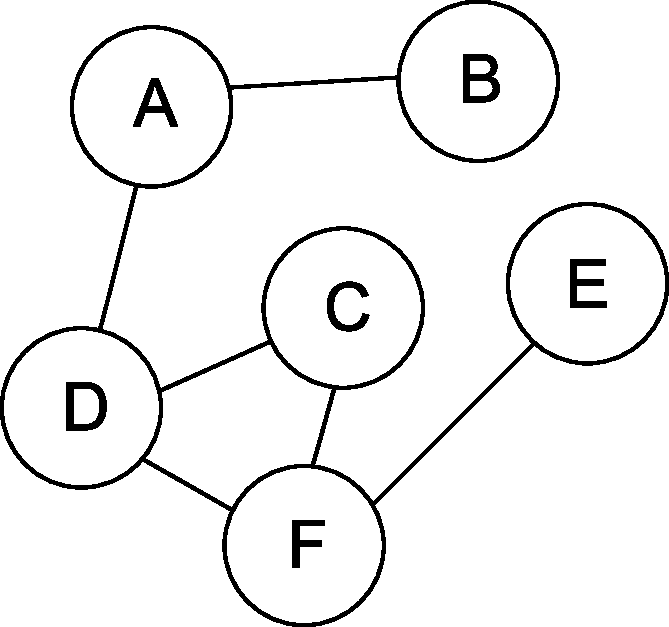
\includegraphics[width=.5\textwidth]{graph.pdf}
\caption{An example graph.}
\label{fig:bfs_dfs_graph}
\end{figure}

Both algorithms start at a root node where the search begins.
In our first example, we will use node D as the root node and E will be our target node.
DFS will visit nodes D, F, and E (in that order).
When we use A as the root node and search for B, DFS will visit nodes A, D, F, E.
At this point, it has gone as deep as it can go and has not found node B.
DFS has to backup and try another branch of nodes.
The algorithm backtracks to node F and tries another route, visiting node C.
Since we have marked node D as already visited, we go no further.
This is important, otherwise DFS will loop infinitely around the cycle in the graph.
We back up again to node F.  We have tried all possible branches from node F, we we back up again to node D.
We have exhausted all sub-branches originating from node D.
We travel back to node A and try any unexplored branches.
We then happen to find node B.

Let's try the same two searches with BFS.
In the first search, we start at node D.
We then search for node B among the neighbors of D, which are nodes A, C, and F.
We still have not found node B, we search among the the neighbors of A, C, and F (that we have not already visited).
We find that node B is a neighbor of node A.
In the second search, we start at node A.  Since node B is a neighbor of node A, we find it immediately.

Both DFS and BFS have advantages.  
If we can choose a root node that is in someway local to the target node, BFS is obviously the better choice.
DFS, in some case, is much more efficient when the solution is far from the target node.
DFS can also be implemented very elegantly as a recursive algorithm (an algorithm that references itself to solve a smaller sub-problem).
However, with large graphs, a recursive algorithm will not perform very well computationally.

\begin{problem}
Implement methods that will perform depth first and breadth first searches on a graph.
Use a \li{set()} to store the visited nodes.  A set data structure supports very efficient membership testing.
Sets are often implemented using binary search trees which have very efficient search characteristics, even with large numbers of elements.

\textit{Hint: The implementations of depth first and breadth first search are exactly same with one very important difference.
The difference is how a particular data structure is used.  What data structure is used differently and how is it used differently?}
\end{problem}
